\documentclass[11pt]{article}

\usepackage{pdfpages}
\usepackage{hyperref}
\usepackage{enumerate}
\usepackage{listings}
\usepackage{float}

\renewcommand*\ttdefault{lmtt}
\renewcommand*\sfdefault{lmss}
\renewcommand{\familydefault}{\sfdefault}

\begin{document}

\author{Group 8}
\title{Laboratory Work 1}
\maketitle

\section{Assignment 1}

\begin{figure}[H]
  \centering
   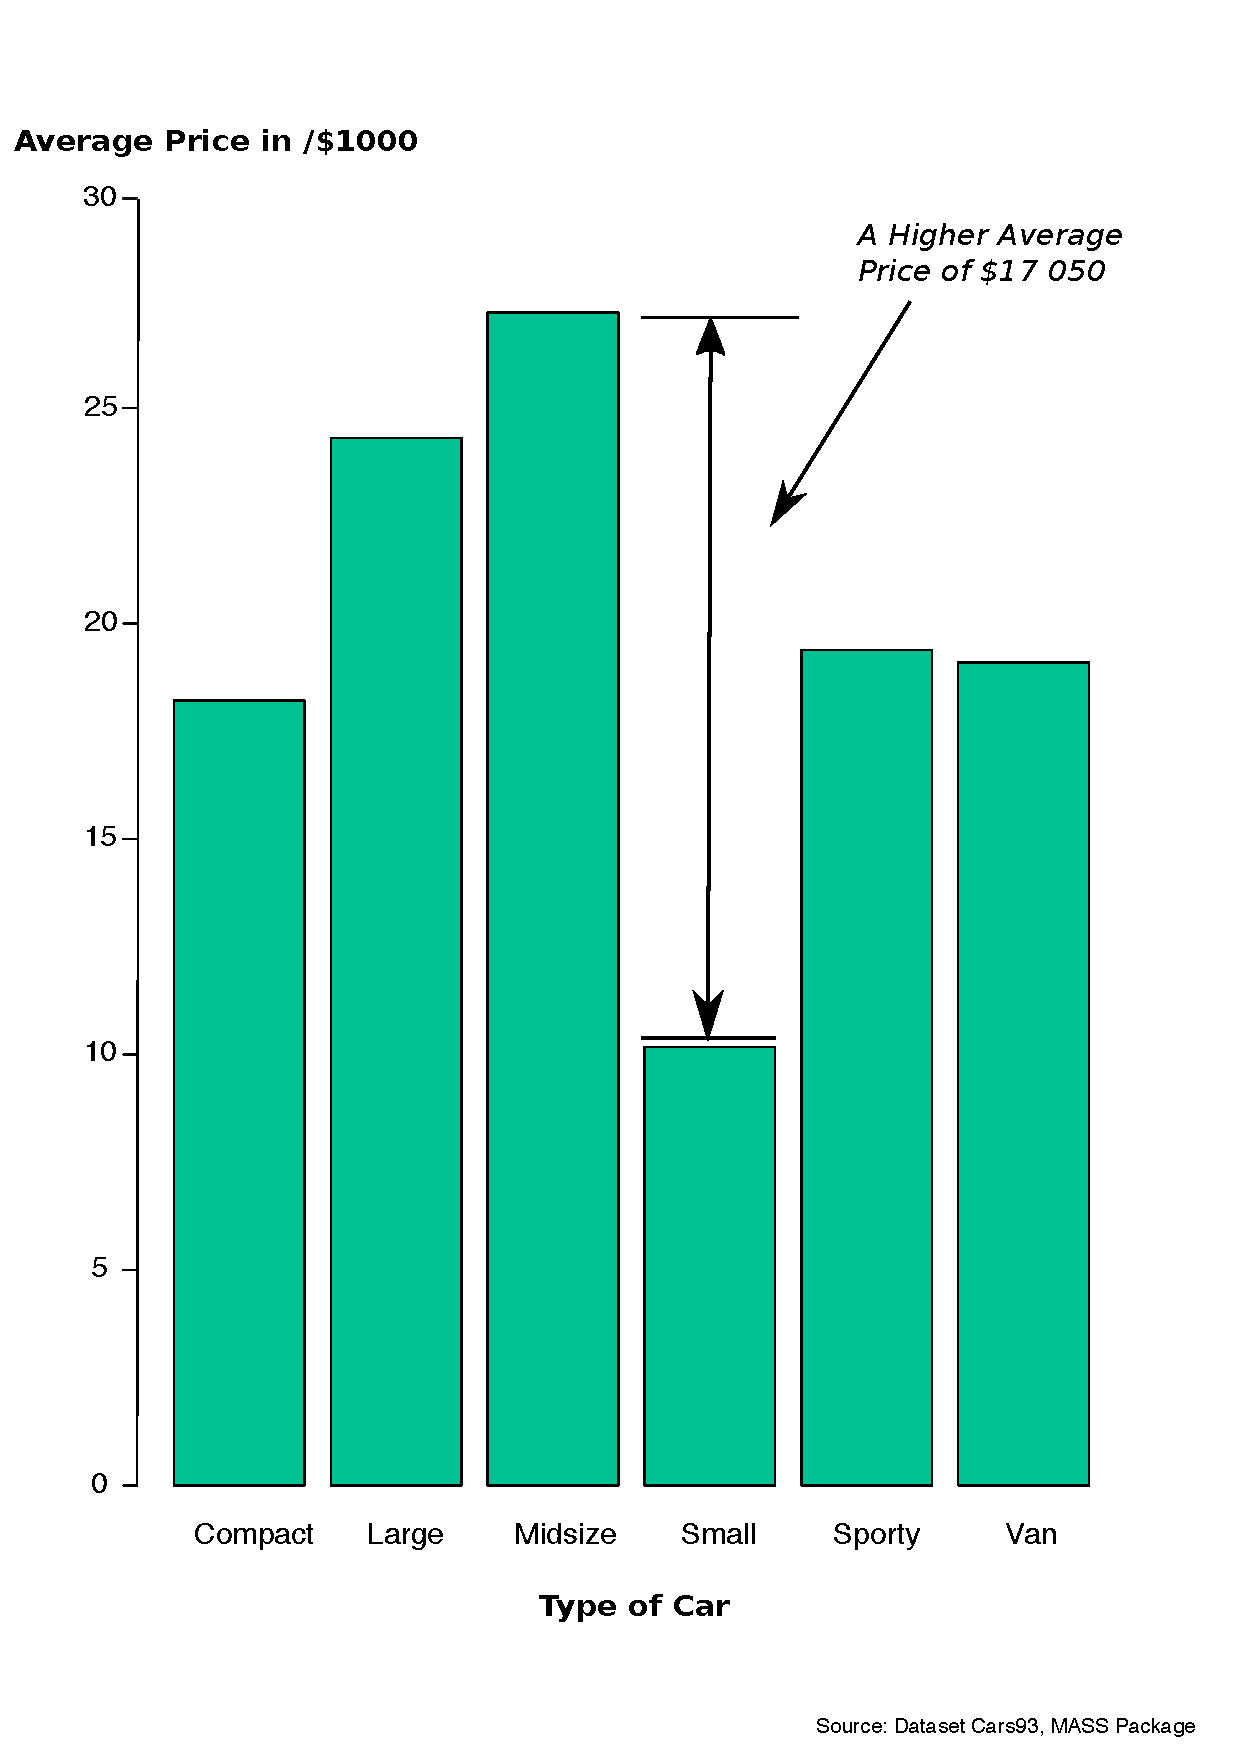
\includegraphics[scale=0.4]{Assignment_1.pdf}
   \caption{The Average Car Price for each type of Car}
\end{figure}


\section{Assignment 2}

\begin{figure}[H]
  \centering
  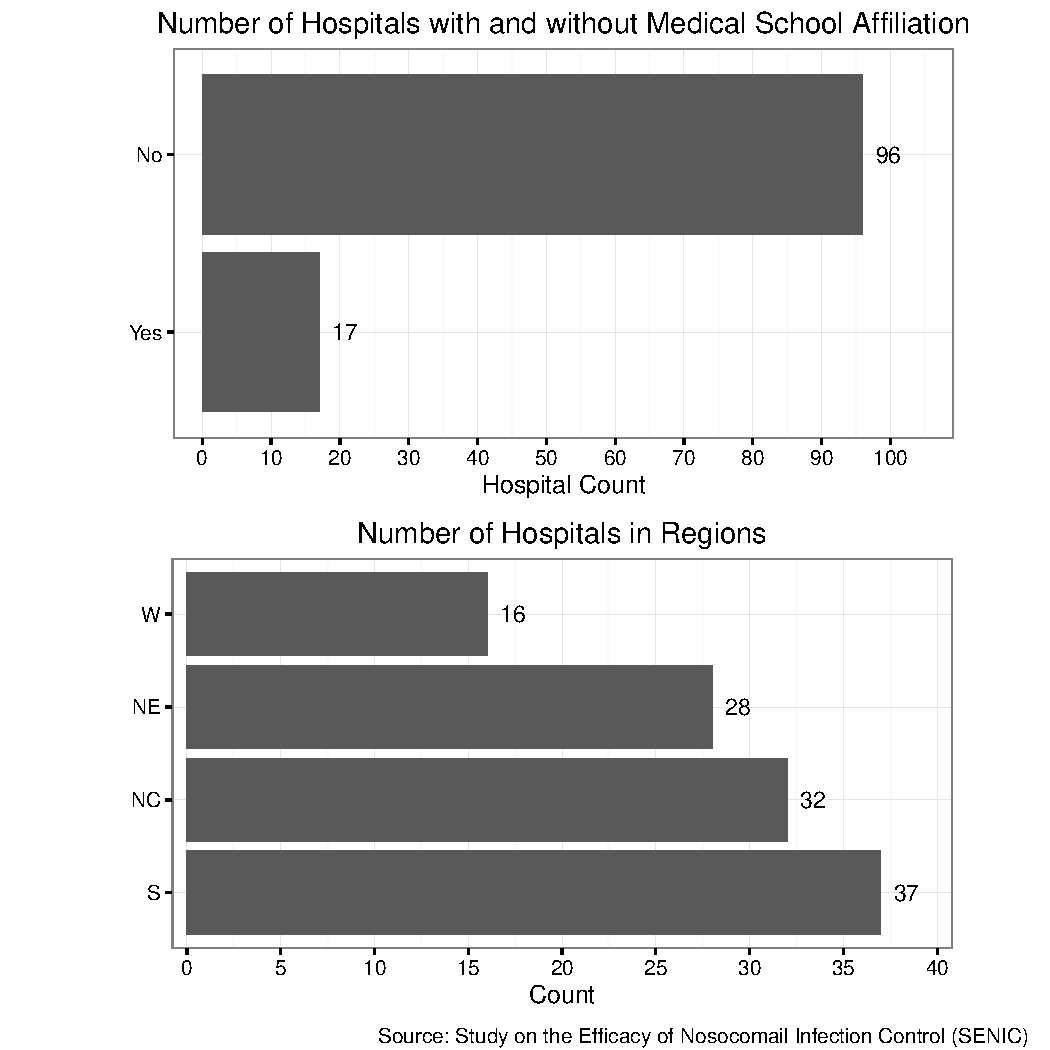
\includegraphics[scale=0.8]{qualitative_vars.pdf}
  \caption{Count of observations of the two
    qualitative variables}
  \label{fig:qualivars}
\end{figure}

There are only two qualitative variables among all: the Medical School
Affiliation (X7) and Region (X8). \autoref{fig:qualivars} is the combined
chart requested.

We can observe from \autoref{fig:qualivars} that
\begin{enumerate}
\item
  Only a few hospitals have affiliation with medical schools.
\item
  The number of hospital in a region varies a lot across regions. This
  does not tell us anything meaningful, however, unless this count is
  normalized by the population size of each regions. So if this is an
  real analysis, the next step may be to construct a graph of the ratio
  'hospital number/population-size', or even better
  'number of bed/population-size'.
\end{enumerate}


\section{Assignment 3}

\begin{figure}[H]
  \centering
   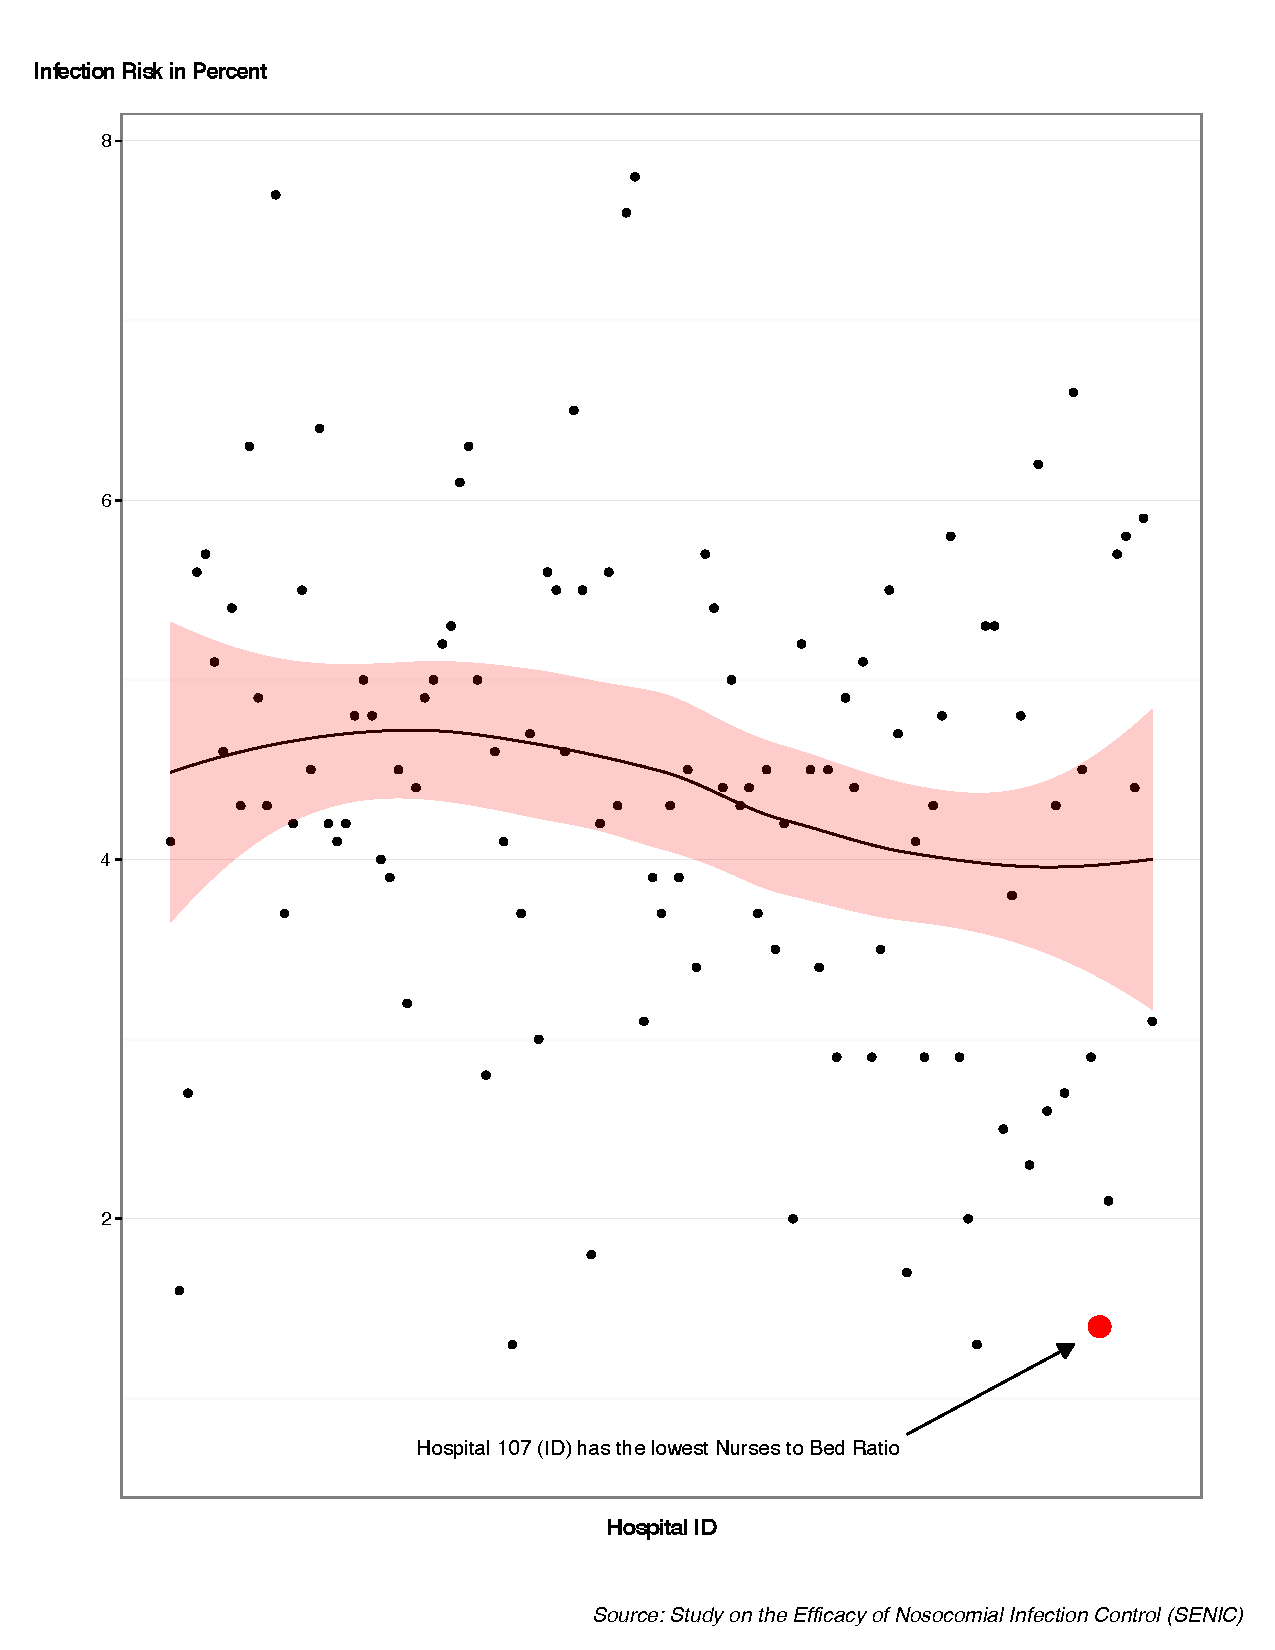
\includegraphics[scale=0.5]{Assignment_3.pdf}
\end{figure}




\end{document}

